\chapter{Numerical Simulation}

\section{Introduction}
In order to get a grasp of the ESG-swap rate process $\kappa_{t}^{ESG}$, we need a model for the ESG-risk score process of the company. It could be logical with a downward trending score since the company will have the incentive to enter such an agreement. 
\\~\\
There are many possible alternatives to model such a model, we impose the following model for the \textbf{ESG-risk score}:
\[
X(t) = 100\exp(-Z(t))
\]

Here $Z(t)$ is an OU-process
\nomenclature{OU}{Ornstein Uhlenbeck}
given by: 
\begin{align*}
dZ(t) &= -\beta Z(t)dt + \sigma dW^{Q}(t) + dI^{Q}(t)    
\end{align*} 
where: 
\begin{align*}
I^{Q}(t) &= \sum_{k=1}^{N(t)}J_{k}, \;\; J_{k}\sim Exp(\mu),\;\; N(t) \sim Pois(\lambda t)    
\end{align*} 

Furthermore $I^{Q}$ and $W^{Q}$ are assumed to be independent, now for $J\sim Exp(\mu)$, we have:
\begin{align*}
f_{J}(x) &= \mu e^{-\mu x}\mathbbm{1}_{[0,\infty)}(x), \;\; 
\E[J] = \frac{1}{\mu}, \;\text{and}\; Var[J] = \frac{1}{\mu^{2}}
\end{align*}

An explicit solution is given by: 
\begin{align}
\label{eq: characteristic_function_Z(t)}
d[e^{\beta t}Z(t)] &= d[e^{\beta t}]Z(t) + e^{\beta t}dZ(t) \nonumber \\ 
&= \beta e^{\beta t}Z(t)dt + e^{\beta t}[-\beta Z(t)dt + 
\sigma dW^{Q}(t) dI^{Q}(t)]
\nonumber \\ 
&=\sigma e^{\beta t}dW^{Q}(t) + e^{\beta t}dI^{Q}(t) \nonumber \\ 
&\Downarrow \nonumber\\ 
Z(t) &= Z(0)e^{-\beta t} +
\int_{0}^{t}e^{-\beta (t-s)}dW^{Q}(s) + 
\int_{0}^{t}e^{-\beta (t-s)}dI^{Q}(s)
\end{align} 



\newpage 

\begin{proposition}[\textbf{Characteristic function of $Z(t)$}]
\label{prop: Characteristic_function_ESG_risk_score}
The characteristic function of $Z(t)$ is given by:
\begin{align*}
\E_{Q}\left[
\exp(iu Z(t))
\right] 
&= 
\exp\left(
iuZ(0)e^{-\beta t}\right)
\left(
-\frac{u^{2}}{4\beta}[1-e^{-2\beta t}]
\right)
\left(
\frac{
1-iue^{-\beta t}1/\mu}
{
1-iu1/\mu
}
\right)^{\frac{\lambda}{\beta}}    
\end{align*}
\end{proposition}

\begin{proof}
Since $I^{Q}$ and $W^{Q}$ are independent we have that: 
\begin{align*}
\E_{Q}[e^{iuZ(t)}]
&= 
\exp\left(
iuZ(0)e^{-\beta t}
\right)
\E_{Q}\left[
\exp\left(
iu\int_{0}^{t}e^{-\beta(t-s)}dW^{Q}(s)
\right)
\right]
\E_{Q}\left[
\exp\left(
iu\int_{0}^{t}e^{-\beta(t-s)}dI^{Q}(s)
\right)
\right]
\end{align*}

The normality of deterministic Ito-integrals gives us:
\begin{align*}
iu\int_{0}^{t}e^{-\beta(t-s)}dW^{Q}(s) &\sim \mathcal{N}\left(
0, -u^{2}\int_{0}^{t}e^{-2\beta(t-s)}ds
\right) \\ 
&\Downarrow \\ 
\E_{Q}\left[
\exp\left(
iu\int_{0}^{t}e^{-\beta(t-s)}dW^{Q}(s)
\right)
\right]
&= 
\exp\left(
-\frac{u^{2}}{4\beta}[1-e^{-2\beta t}]
\right)
\end{align*}

From Proposition \ref{prop: Integral_g(s)dI(s)} (p.\pageref{prop: Integral_g(s)dI(s)}), we have: 
\begin{align*}
\E\left[
\exp\left(iu\int_{0}^{t}e^{-\beta(t-s)}dI(s)\right)
\right] 
&= 
\exp\left(
\int_{0}^{t}\Psi(ue^{-\beta s})ds
\right)
\end{align*}

To ease some notation, we write:
\begin{align*}
\Psi(x) &= \lambda(\varphi_{F}(x) - 1), \;\text{where:}\; 
\varphi_{F}(x) = \int_{\R}e^{iyx}F_{J}(dy) 
\end{align*}

We start with calculating $\varphi_{F}(x)$ with $F_{J}(dy) = 
\mu e^{-\mu y}\mathbbm{1}_{[0,\infty)}(y)dy:$ 
\begin{align*}
\varphi_{F}(x) &= 
\int_{0}^{\infty}e^{ixy}\mu e^{-\mu y}dy   
= \frac{1}{1-ix\frac{1}{\mu}}
\end{align*}

Giving us:
\begin{align*}
\varphi_{F}(x) - 1
= 
\frac{1}{1-ix\frac{1}{\mu}} - \frac{1-ix\frac{1}{\mu}}{1-ix\frac{1}{\mu}} 
= 
\frac{ix\frac{1}{\mu}}{1-ix\frac{1}{\mu}}
\end{align*}

Now: 
\begin{align*}
\Psi(ue^{-\beta s}) &= \lambda(\varphi_{F}(ue^{-\beta s})) -1) \\ 
&= \lambda\left(
\frac{iue^{-\beta s}1/\mu}{1-iue^{\beta s}1/\mu}
\right)\cdot \frac{\beta}{\beta} \\ 
&= 
\frac{\lambda}{\beta}\left(
\frac{\beta iue^{-\beta s}1/\mu}{1-iue^{\beta s}1/\mu}
\right)
\end{align*}

\newpage 
We observe: 
\begin{align*}
h(s) :&= \ln[1-iue^{-\beta s}1/\mu] \\ 
&\Downarrow \\ 
h'(s) &= \frac{\beta iue^{-\beta s}1/\mu}{1-iue^{\beta s}1/\mu} 
\end{align*}

Leaving us with: 
\begin{align*}
\int_{0}^{t}\Psi(ue^{-\beta s})ds
&= 
\frac{\lambda}{\beta}\int_{0}^{t}h'(s)ds
= 
\frac{\lambda}{\beta}[h(t)-h(0)] 
= 
\frac{\lambda}{\beta}
\ln\left[
\frac{1-iue^{-\beta t}1/\mu}{1-iu1/\mu}
\right]
\end{align*}

\end{proof}


By using Proposition \ref{prop: Characteristic_function_ESG_risk_score} we can find the expectation of $X(t)$: 
\begin{align*}
\E_{Q}\left[X(t)\right]
&= 
\E_{Q}\left[
e^{i(-i)Z(t)}
\right] \\ 
&= 
\exp\left(
Z(0)e^{-\beta t}
\right)
\exp\left(
\frac{1}{4\beta}[1-e^{-2\beta t}]
\right)
\left(
\frac{
1 + e^{-\beta t}1/\mu
}{
1 + 1/\mu
}
\right)
\end{align*}

Now if $\beta > 0$, one can find: 
\begin{align*}
\lim\limits_{t \to \infty}\E_{Q}[X(t)]
&= 
\exp\left(
\frac{1}{4\beta} + \frac{1}{1+1/\mu}
\right)
\end{align*}

\begin{figure}[htp]
    \centering
    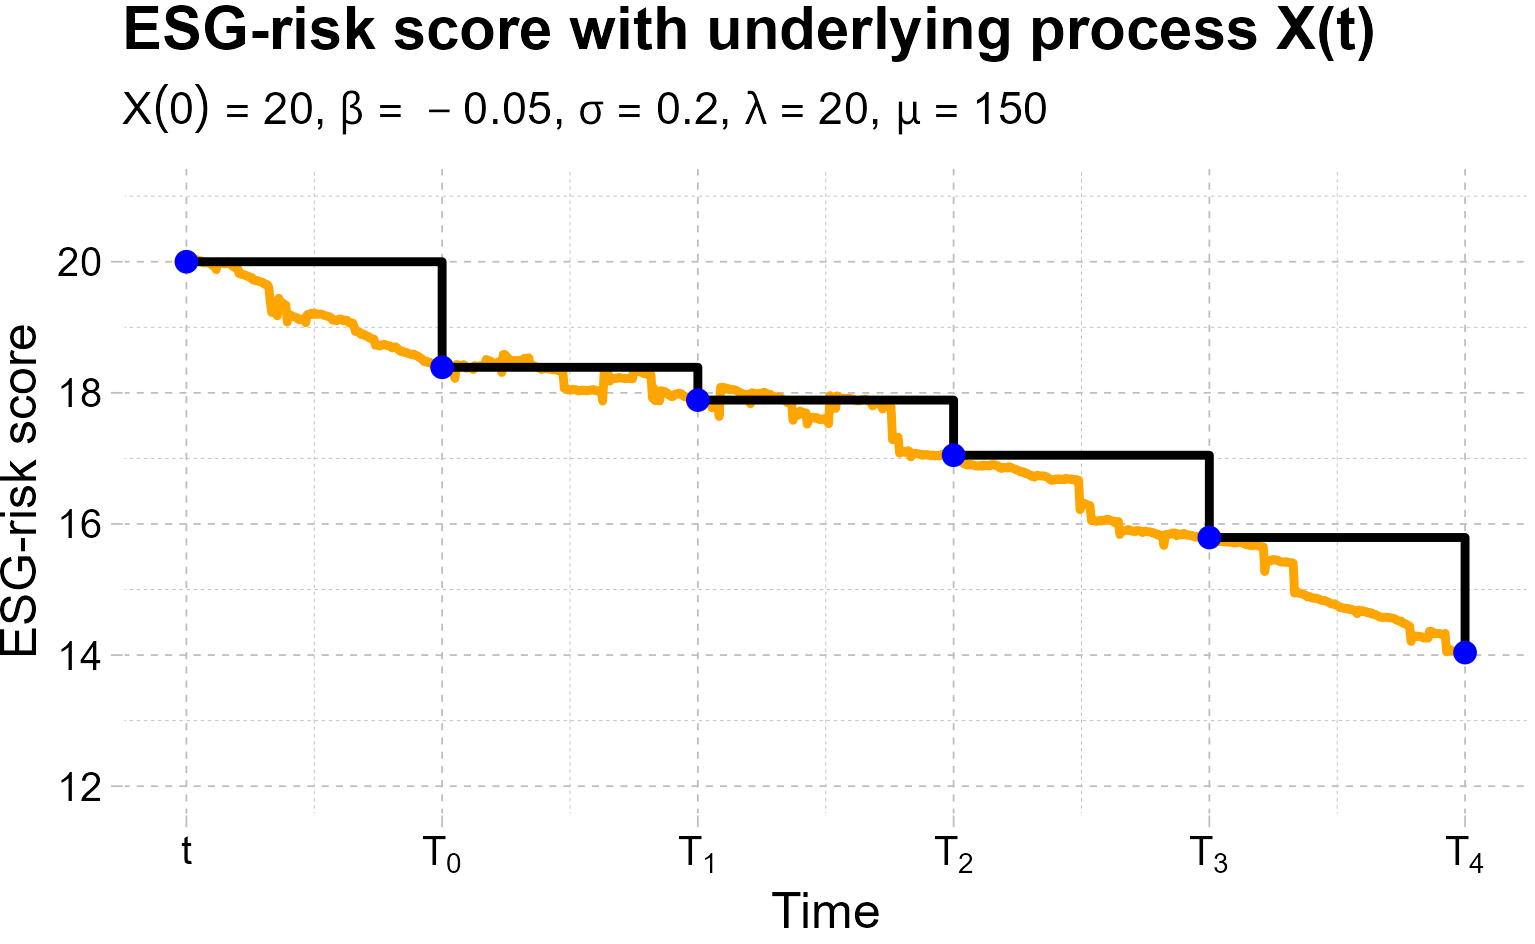
\includegraphics[width=11cm]{figures/ESG/Trajectory_X(t)_params.png}
    \caption{ESG-risk score with underlying process $X(t)$}
    \label{fig: ESG_risk_score_underlying_X(t)}
\end{figure}

The blue dots represent the observed ESG-risk score at the relevant observation times. The solid dark line represents the ESG-risk score between observation times, and the orange underlying process represents our continuous time ESG-risk score process $X(t)$.  

\newpage 

\section{Simulation of Zero Coupon Bond ESG-swap}

In this section, we will look at a numerical simulation of the ESG-swap rate process $\kappa_{t}^{ESG} = (\kappa_{t}^{ESG}(i))_{i=1, \dots, 4}$. We will simulate different scenarios, these will be when the ESG-criteria $C^{ESG}$ is reasonable, and when the ESG criteria are unreasonable. 
\\~\\
By unreasonable we will look at the extremes, i.e where the criteria are met all the time, and where the criteria are never met. This will show the effect of the discount and penalty respectively. 
\\~\\ 
Assume that after analysis one has arrived at the conclusion that the model as described in Figure \ref{fig: ESG_risk_score_underlying_X(t)} is a good fit for the counterparty company in this ESG-swap. 
\\~\\
\textbf{Parameters}
\begin{itemize}
    \item $X(0) = 20 \implies Z(0) = -\ln\left(\frac{20}{100}\right)$
    \item $\beta = -0.05$
    \item $\sigma = 0.2$
    \item $\lambda = 20$
    \item $\mu = 150$
\end{itemize}

We will use a stepsize of $dt = \frac{1}{360}$, and since the calculation is based upon Monte Carlo simulations, we will base the calculation on 1 Million simulations ($n\_sim = 10^{6})$. 
\\~\\ 
\textbf{Agreement/specifications}
\begin{itemize}
    \item For simplicity we will assume that our ESG criteria process $C^{ESG} = (C^{ESG}_{T_{i}})_{
    \{i=1, \dots, 4\}}$ to be $\F_{0}$-measurable. 
    \item $\delta = 1$ meaning that the time between observations times $T_{i}$ and $t_{i-1}$ is one year. 
    \item We assume that the penalty/discount $d = 0.005$.
    \item We will also for simplicity set: 
    \[
    \kappa_{t}^{ZCB} = \frac{P(t,T_{0})-P(t,T_{4})}{\delta \sum_{i=1}^{4}P(t,T_{i})} = 0.07
    \]
\end{itemize}
\newpage 

\textbf{Reasonable criteria}
\begin{itemize}
    \item $C^{ESG} = (17.6, 16.6, 15.6, 14.55)$
\end{itemize}



\newpage 


\textbf{Agreement}: 
\begin{itemize}[leftmargin =*]
    \item We agree upon $C^{ESG} = (C_{T_{i}}^{ESG})_{i\in \{1,2,3,4\}} = (17.6, 16.6, 15.6, 14.55)$ 
    \item One evaluates the ESG-risk score at $(T_{1}, T_{2}, T_{3}, T_{4}) = (1.25, 2.25, 3.25, 4.25)$
\end{itemize}

\textbf{Parameters}:
\begin{itemize}
    \item $d = 0.005$
    \item $\delta = 1$
    \begin{align*}
    \left(
    Z(0) = -\ln(\frac{20}{100}), \beta = -0.05, \lambda = 20, \mu = 150, \Delta t = \frac{1}{360}
    \right)   
\end{align*} 
    \item \begin{align*}
        \left(
        P(t,T_{0}) = 0.995, P(t,T_{1}) = 0.985, P(t,T_{3}) = 0.975, P(t,T_{4}) = 0.965
        \right)
    \end{align*}
    \item Number of simulations: $10^{6}$
\end{itemize}

We assume that the dynamics under $Q$ look the following: 
\begin{figure}[htp]
    \centering
    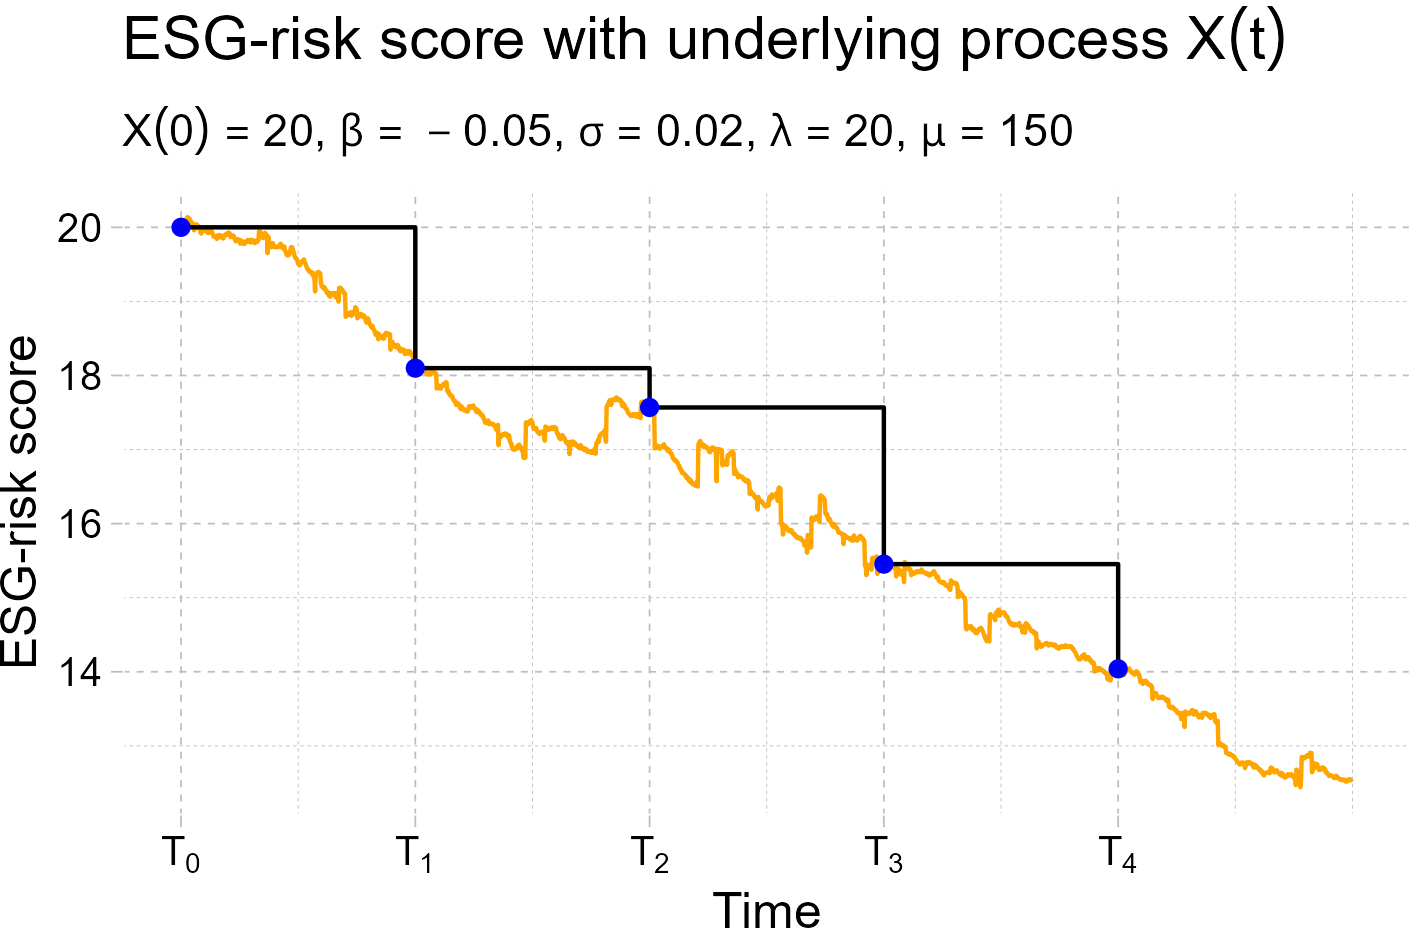
\includegraphics[width=10cm]{figures/ESG/ESG_OU_path.png}
    \caption{trajectory of $X(t)$}
    \label{fig: ESG-risk score}
\end{figure}

This graph indicates that the ESG-risk score is downward trending, this could be that the company are/will implement measures to reduce $CO_{2}$-emissions.
The blue dots represent the ESG-risk score at times $T_{i}$. 


\newpage 

In this simulation we got: 
\begin{align*}
\kappa_{t}^{ZCB} &= \frac{P(t,T_{0})-P(t,T_{4})}{\delta \sum_{i=1}^{4}P(t,T_{i})} = 0.01030   
\end{align*}

\begin{figure}[htp]
    \centering
    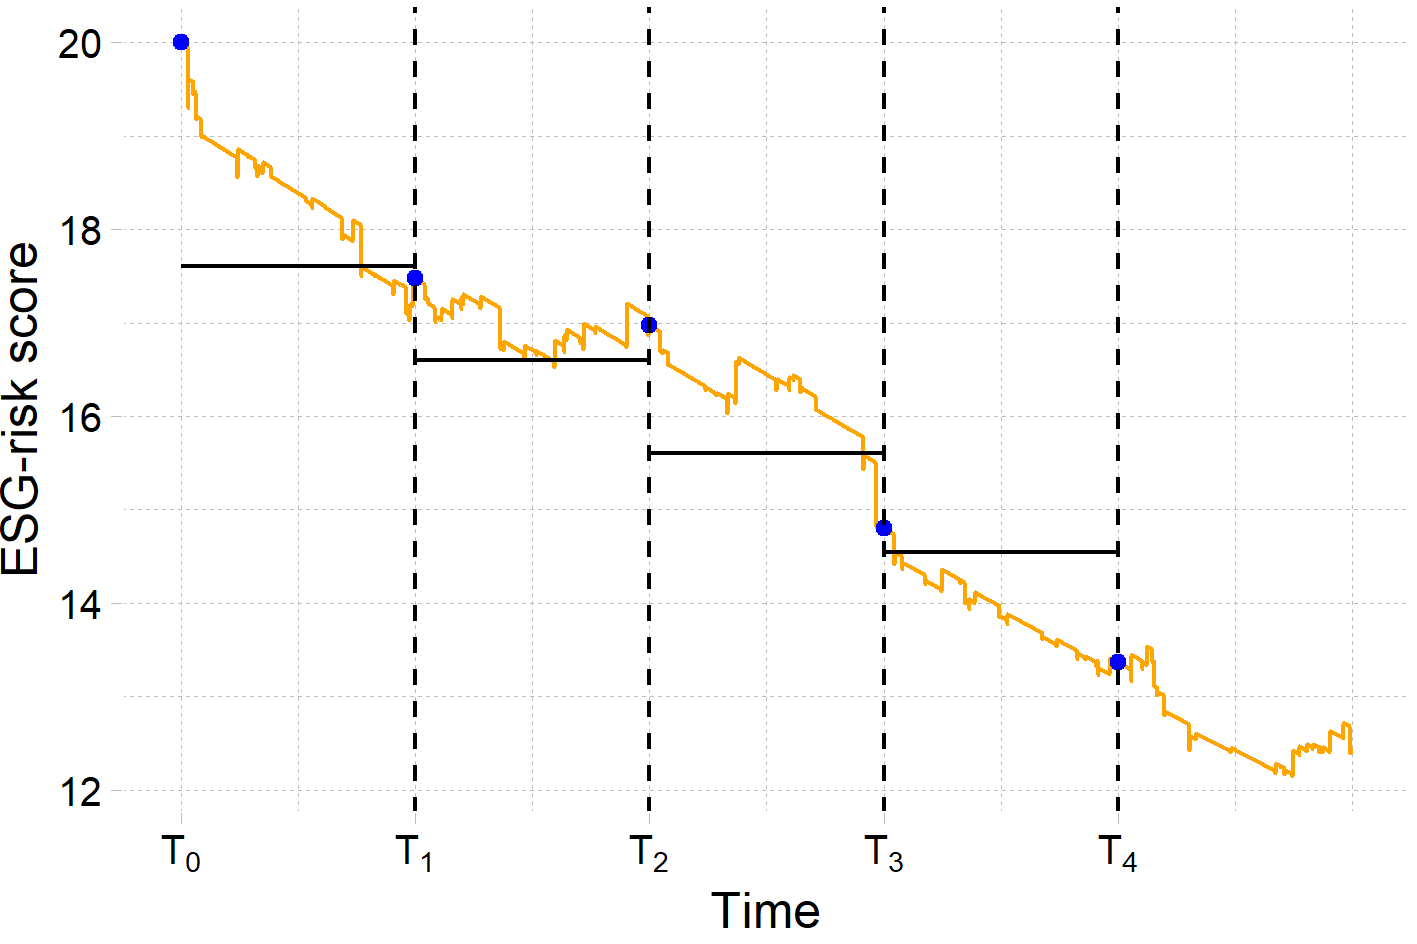
\includegraphics[width= 9cm]{figures/ESG/ESG_plt_criteria.png}
    \caption{ESG-risk score where ESG-criteria is reasonable}
    \label{fig: ESG-risk_criteria1}
\end{figure}

In this figure, we see the underlying ESG risk score process. Here the dark-solid lines represent the criteria $C_{T_{i}}^{ESG}$. We see that the ESG criteria were bearly met at time $T_{1}$, it was not met at $T_{2}$, met at $T_{3}$ and then met again at time $T_{4}$. 
\\~\\ 
We summarize the findings in the following table:
\begin{center}
    \begin{tabular}{ | l | l | l | p{5cm} |}
    \hline
    Time    &   Criteria  & $\kappa_{t}^{ESG}(i)$ \\ \hline
    $T_{1}$ &      17.6   & $0.01224$  \\ \hline
    $T_{2}$ &      16.6   & $0.01119$  \\ \hline
    $T_{3}$ &      15.6   & $0.01023$  \\ \hline
    $T_{4}$ &      14.55  & $0.00780$   \\ \hline
    \end{tabular}
\end{center} 

\begin{figure}[htp]
    \centering
    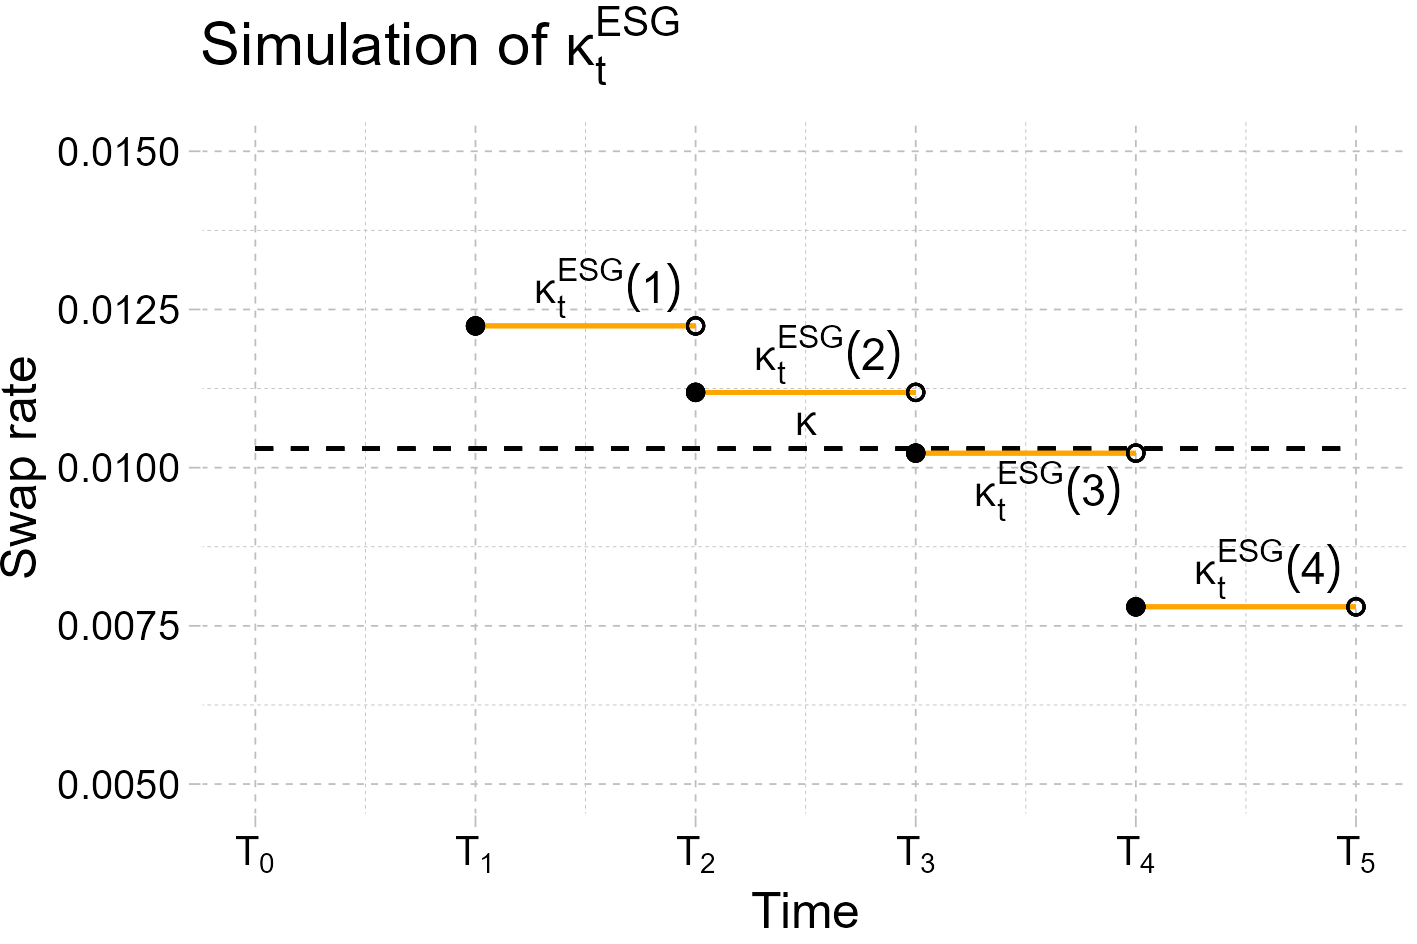
\includegraphics[width= 10cm]{figures/ESG/kappa_t_ESG_1.png}
    \caption{ESG-risk score where ESG-criteria is reasonable}
    \label{fig: ESG_swap_1}
\end{figure}

\newpage 

\textbf{Meeting criteria often}
\\~\\ 
In this simulation we took: $C^{ESG} = (18,17,16,15)$, and we got the following: 

\begin{figure}[htp]
    \centering
    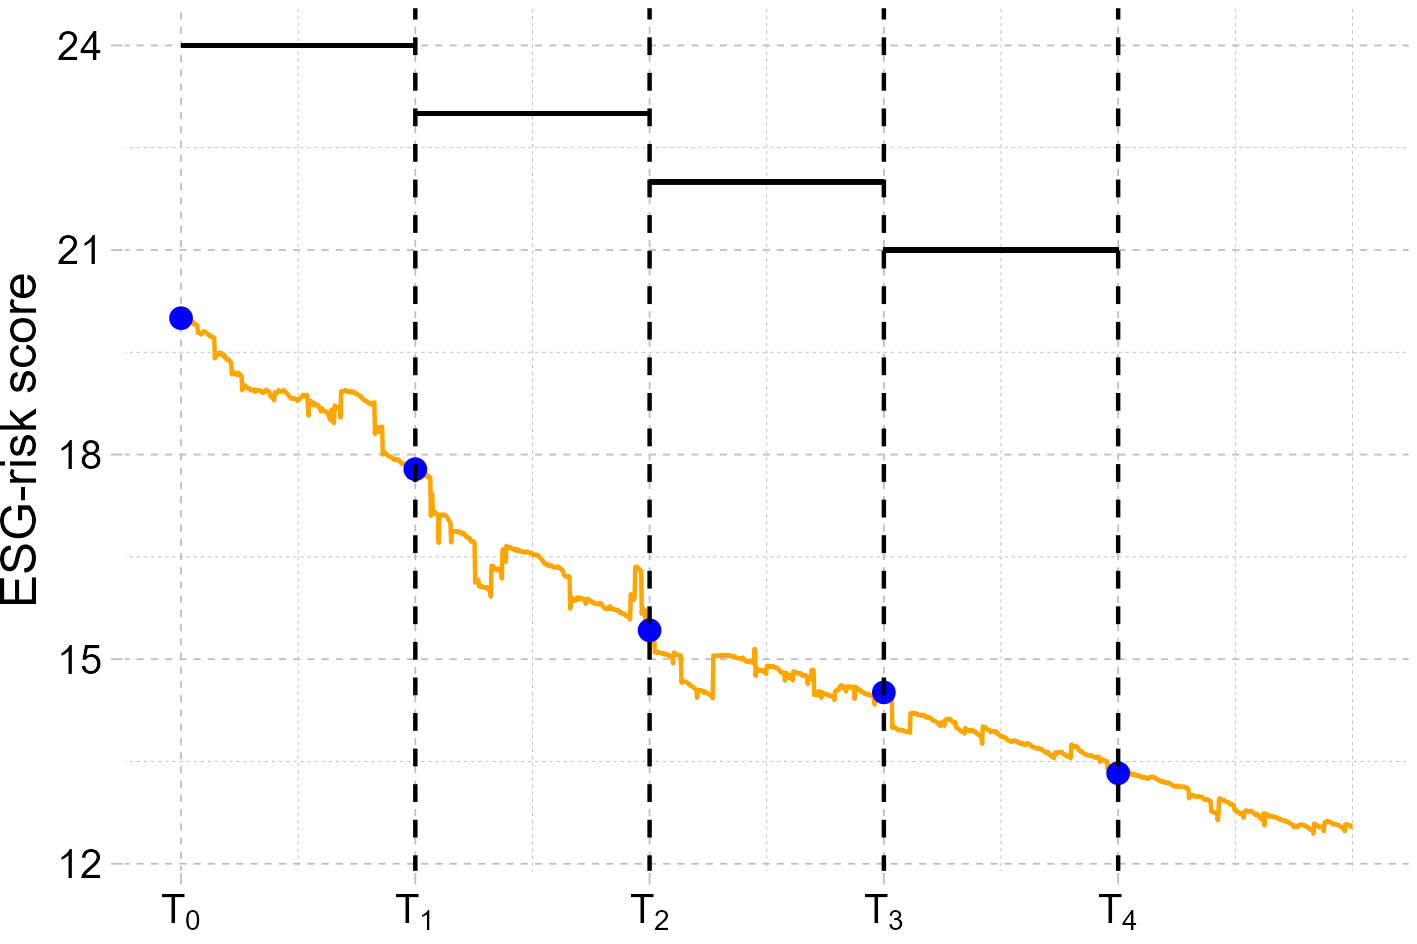
\includegraphics[width= 9cm]{figures/ESG/ESG_plt_criteria2.png}
    \caption{ESG-risk score where ESG-criteria is met often}
    \label{fig: ESG-risk_score_criteri2}
\end{figure}

In this particular we met the criteria at all time points $T_{i}$ for $i=1,2,3$. 


\begin{center}
    \begin{tabular}{ | l | l | l | p{5cm} |}
    \hline
    Time    & Criteria   & $\kappa_{t}^{ESG}(i)$ \\ \hline
    $T_{1}$ &   18       & $0.01046$  \\ \hline
    $T_{2}$ &   17       & $0.00876$  \\ \hline
    $T_{3}$ &   16       & $0.00605$\\ \hline
    $T_{4}$ &   15       & $0.00273$ \\ \hline
    \end{tabular}
\end{center} 

\begin{figure}[htp]
    \centering
    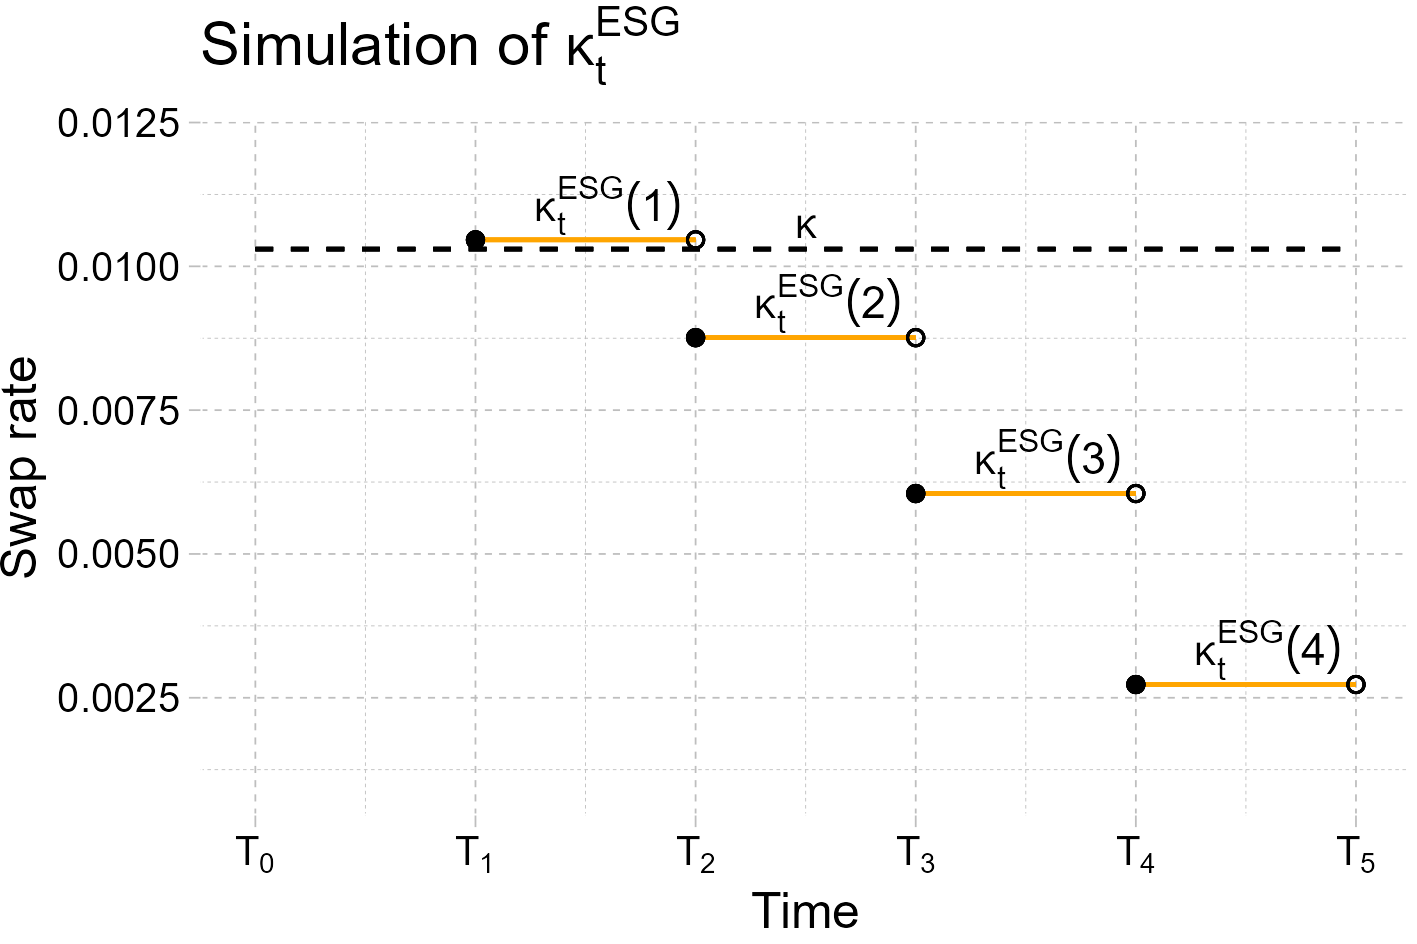
\includegraphics[width= 10cm]{figures/ESG/kappa_t_ESG_2.png}
    \caption{Meeting criteria often}
    \label{fig: ESG_swap_2}
\end{figure}

In this simulation, we got almost the swap rate at time $T_{1}$, and then the company met the criteria for $i=2,3,4$, giving a lower fixed rate. 


\newpage
\textbf{Never meeting criteria}
\\~\\ 
In this simulation we took: $C^{ESG} = 2.5$, for all timepoints and got: 

\begin{figure}[htp]
    \centering
    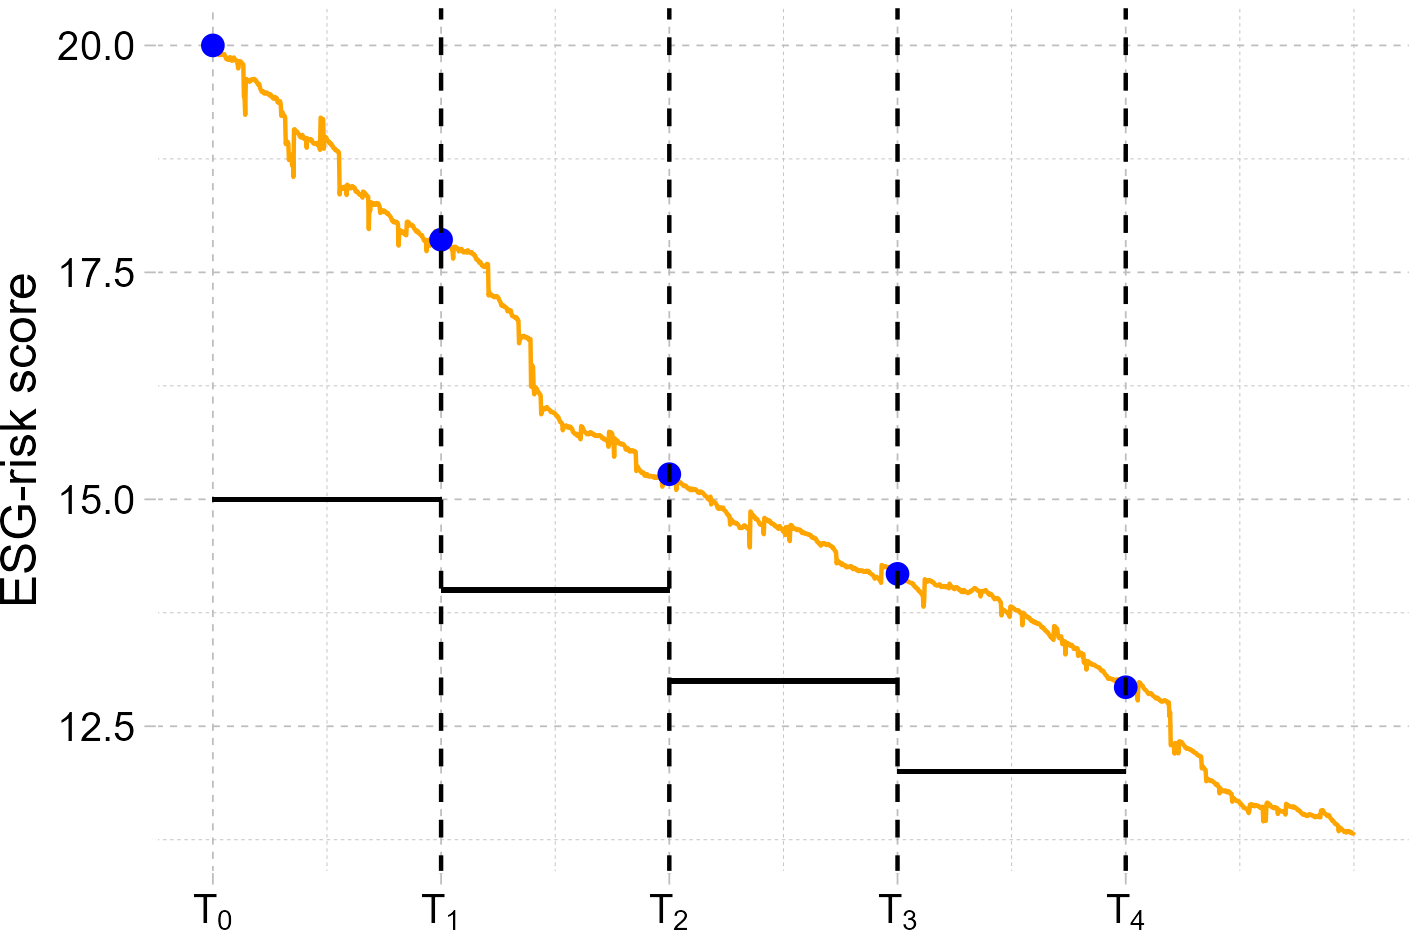
\includegraphics[width=9cm]{figures/ESG/ESG_plt_criteria3.png}
    \caption{ESG-risk score where ESG-criteria is never met}
    \label{fig: ESG-risk_score_criteria3}
\end{figure}




\begin{center}
    \begin{tabular}{ | l | l | l | p{5cm} |}
    \hline
    Time    & Criteria  & $\kappa_{t}^{ESG}(i)$ \\ \hline
    $T_{1}$ &    2.5    & $0.0153$  \\ \hline
    $T_{2}$ &    2.5    & $0.0203$  \\ \hline
    $T_{3}$ &    2.5    & $0.0253$\\ \hline
    $T_{4}$ &    2.5    & $0.0303$ \\ \hline
    \end{tabular}
\end{center} 


\begin{figure}[htp]
    \centering
    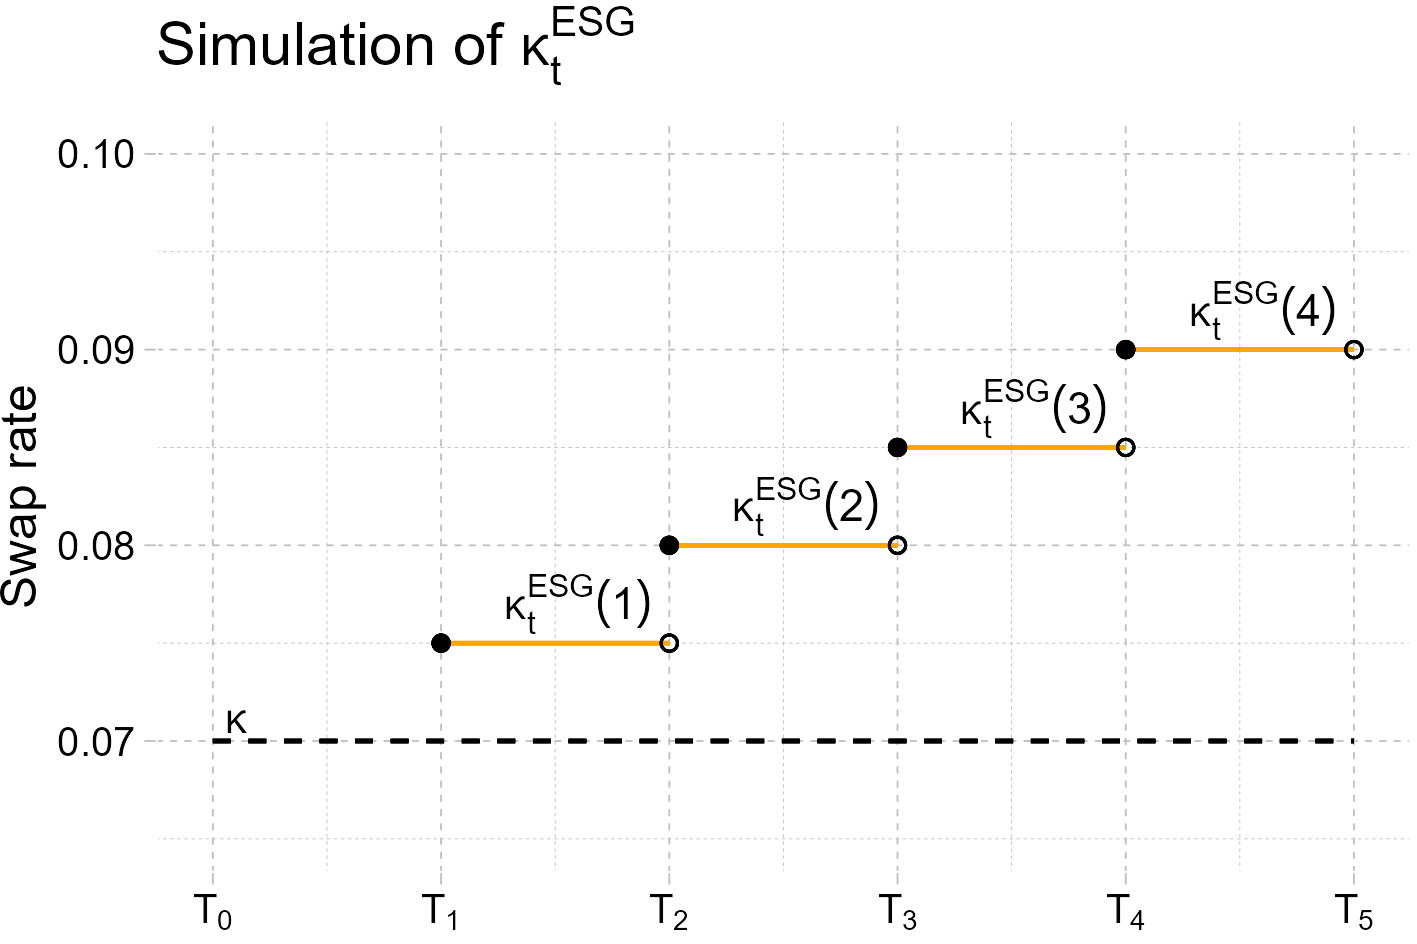
\includegraphics[width=10cm]{figures/ESG/kappa_t_ESG_3.png}
    \caption{ESG swap rate when ESG-criteria is never met}
    \label{fig: ESG_swap_3}
\end{figure} 

We see the effect of the penalty $d = 0.005$, leading to an upward-trending ESG swap rate. 









